% This is LLNCS.DOC the documentation file of
% the LaTeX2e class from Springer-Verlag
% for Lecture Notes in Computer Science, version 2.4
\documentclass{llncs}
\usepackage{llncsdoc}
\usepackage{graphicx}
\usepackage{amssymb}
\usepackage[table]{xcolor}
%\usepackage[cp1250]{inputenc} % WH
%\usepackage[polish]{babel}    % WH

% Added for code listing
\usepackage{listings}
\usepackage{caption}

\newcounter{nalg}[chapter] % defines algorithm counter for chapter-level
\renewcommand{\thenalg}{\thechapter .\arabic{nalg}} %defines appearance of the algorithm counter
\DeclareCaptionLabelFormat{algocaption}{Algorithm \thenalg} % defines a new caption label as Algorithm x.y

\lstnewenvironment{algorithm}[1][] %defines the algorithm listing environment
{
    \refstepcounter{nalg} %increments algorithm number
    \captionsetup{labelformat=algocaption,labelsep=colon} %defines the caption setup for: it ises label format as the declared caption label above and makes label and caption text to be separated by a ':'
    \lstset{ %this is the stype
        frame=tB,
        numbers=left,
        numberstyle=\tiny,
        basicstyle=\scriptsize,
        keywordstyle=\color{black}\bfseries\em,
        keywords={,input, output, return, datatype, function, in, if, else, foreach, while, begin, end, done, } %add the keywords you want, or load a language as Rubens explains in his comment above.
        numbers=left,
        xleftmargin=.04\textwidth,
        #1 % this is to add specific settings to an usage of this environment (for instnce, the caption and referable label)
    }
}
{}

\usepackage{url}
\urldef{\mailwhajwp}\path|{xxx,yyy,zzz}@mini.pw.edu.pl|
\newcommand{\keywords}[1]{\par\addvspace\baselineskip
\noindent\keywordname\enspace\ignorespaces#1}
%
\begin{document}


% first the title is needed
\title{Pattern Recognition with Rejection}
\subtitle{Combining Standard Classification Methods\\with Geometrical Rejecting}

% a short form should be given in case it is too long for the running head
\titlerunning{Pattern Recognition with Rejection}
%

\author{Wladyslaw Homenda\inst{1,2}, Agnieszka Jastrzebska\inst{1}, Piotr Waszkiewicz\inst{1}\\ and Anna Zawadzka\inst{1}}
%
\authorrunning{W. Homenda et. al}
% (feature abused for this document to repeat the title also on left hand pages)

% the affiliations are given next; don't give your e-mail address
% unless you accept that it will be published
\vspace{-6pt}
\institute{Faculty of Mathematics and Information Science, Warsaw University of Technology\\
ul. Koszykowa 75, 00-662 Warsaw, Poland \and Faculty of Economics and Informatics in Vilnius, University of Bialystok\\Kalvariju g. 135, LT-08221 Vilnius, Lithuania
}
\vspace{-6pt}
\maketitle
\vspace{-6pt}

\pagestyle{empty}  % no page numbers, no running headers

\begin{abstract}
\vspace{-12pt}
The motivation of our study is to provide algorithmic approaches to distinguish proper patterns, from garbage and erroneous patterns in a~pattern recognition problem. The design assumption is to provide methods based on proper patterns only. In this way the approach that we propose is truly versatile and it can be adapted to any pattern recognition problem in an uncertain environment, where garbage patterns may appear. The proposed attempt to recognition with rejection combines known classifiers with geometric methods used for separating native patterns from foreign ones. Empirical verification has been conducted on datasets of handwritten digits classification (native patterns) and handwritten letters of Latin alphabet (foreign patterns).
\vspace{-6pt}
\keywords pattern recognition, classification, rejecting option, geometrical methods
\vspace{-6pt}
\end{abstract}


%\end{document}
\vspace{-12pt}
%-------------------------------------------------------------------
%-------------------------------------------------------------------
%-------------------------------------------------------------------
\section{Introduction}
  \label{sec:Introduction}
\vspace{-3pt}

The task of pattern recognition is a classical machine learning problem. As an input we pass a training dataset, consisting of labelled patterns belonging to $c$~classes. In the process we expect to form a model that assigns correct labels to new patterns (new observations).

It is important to have in mind that patterns in their original form are often some sort of signal, for instance images or voice recordings. Due to the fact that the original patterns are often collected using some signal-acquiring devices, we may encounter patterns that do not belong to any of the proper classes. Such situation may happen, when the device that we have used to acquire data has been automatically reset due to power outage and poor default calibration distorts the segmentation process. Another scenario is when we collect data in a noisy (out of lab) environment and apart from proper patterns there are a lot of unexpected residual ones. The problem with such patterns, say -- garbage patterns, is that we cannot predict their characteristics and therefore we cannot include information about them in the model training process.

The motivation for our study is to provide algorithmic approaches used for distinguishing proper patterns, that we call \textit{native patterns} from garbage and erroneous patterns, that we call \textit{foreign patterns}. The task described in this paper we call \textit{foreign patterns rejection}. The design assumption is to provide methods based on native patterns only. In this way the framework that we propose is truly versatile and it can be adapted to any pattern recognition problem in an uncertain environment, where foreign patterns may appear. 

The study focuses on designing methods for recognition with rejection and employs them to (a) distinguish native patterns from foreign ones and (b) improve classification quality of native patterns. A specific objective of this study is to examine the cooperation of various standard classifiers (SVMs, random forests and kNNs) with geometric methods used for rejection. We focus on the influence of rejection mechanisms on native patterns classification, i.e., improvement of Fine Accuracy measure. The proposed methods are empirically verified on datasets of handwritten digits (native patterns) and handwritten Latin letters (foreign patterns).

We would like to emphasise that the novelty of the contribution presented in this paper is not in the methods that we use, but in how we employ them and on what we achieve with them.  %We also test the effectiveness of foreign patterns rejection and differences between used classifiers. %TODO koniecznie trzeba dodac wiecej opisu novelty/objective, dodamy na koncu jak bedzie calosc artykulu 

The remainder of this paper is organized as follows. Section \ref{sec:Literature Review} presents the background knowledge on foreign patterns detection present in the literature. Sections~\ref{sec:Ellipsoids} and~\ref{sec:Classifiers} present the backbone algorithms, known in the literature, that we use to construct our models. Section \ref{sec:Methodology} presents the proposed approach. In Section \ref{sec:Experiments} we discuss a series of experiments. % based on images of handwritten digits. 
Section \ref{sec:Conclusion} concludes the paper and highlights future research directions.
%Lastly, Section \ref{sec:Conclusion} concludes the paper and highlights future research directions.


\vspace{-3pt}
%-------------------------------------------------------------------
%-------------------------------------------------------------------
%-------------------------------------------------------------------
\section{Preliminaries}
  \label{sec:Preliminaries}
\vspace{-6pt}

Data collection and processing are vital study problems across multiple domains of science. Along with a substantial automation of data acquisition we face difficulties that appear due to poor data quality. The research we present in this paper has been motivated by the issue of contaminated datasets, that apart from proper patterns contain garbage.

In this section we start the discussion with a review of relevant literature positions in machine learning that tackle the issue of contaminated datasets. Then, in order to provide a self-contained description of the employed methods we present backbone literature algorithms applied. In what follows we present the Minimum Volume Enclosing Ellipsoid (MVEE) algorithm and a suite of three classification methods: Random Forests (RF), Support Vector Machines (SVM), and K-Nearest Neighbors algorithm (kNN). Listed methods are employed in various configurations to native patterns classification with foreign patterns rejection. Our approach, based on those algorithms, is discussed in Section \ref{sec:Methodology}.


\vspace{-6pt}
%-------------------------------------------------------------------
%-------------------------------------------------------------------
\subsection{Literature Review}
  \label{sec:Literature Review}
\vspace{-3pt}

The rejecting option in pattern recognition problem has gained a rather weak attention despite its importance in practice. Also, there is a~relatively short list of papers raising the problem of rejecting foreign patterns, cf.~\cite{HomendaICAART2015} for a~short survey. % In this paper we study several attempts to classification with rejection of foreign patterns. Scenarios for the discussed methods is based on well-known combinations of machine learning algorithms.  
Here we only hint some issues present in literature. Due to space limitations we are neither able to comprehensively cover the subject, nor can we provide a~deep background of the methods employed in this study.

Discussion on approaches related to foreign patterns rejection may start with one-class classification methods. Especially, there are two noteworthy examples: centroid-based methods and One-Class Support Vector Machine.

Centroid-based methods rely on distinguishing cluster centres (centroids). Region reserved for proper patterns is usually defined by the distance between centre and the furthest proper pattern.

One-Class SVM has been introduced in \cite{ScholkopfWilliamsonSmola1992}. While ``regular'' SVM algorithm forms hyperplane separating two classes, the One-Class SVM separates data points from the entire feature space. Notably, the One-Class SVM provides a soft decision rules, as there is a $\nu$ parameter determining the fraction for outliers.  

%It is worth to emphasize the analogy between outlier detection and foreign patterns rejection. However, the motivation for those two problems remains different.

When it comes to the study on actual foreign patterns rejection, there are relatively few papers to review. This issue, in spite of its importance, remains somehow neglected. Among notable studies one may mention rank-based methods, for instance ones described in \cite{BertolamiZimmermannBunke2006,BurgerKessentiniPaquet2011,EladHel-OrKeshet2001,HempstalkFrankWitten2008,SchemeHudginsEnglehart2013,TaxDuin2008,WangCasasent2009}.
In a nutshell, mentioned papers propose to attach confidence scores along with class labels. Rejection occurs when none of native class labels was assigned with a satisfying confidence.

%In our paper we assume an approach that in its background resembles more model-based outlier detection techniques than reported in the literature foreign patterns rejection schemes. The objective of our study is to form a model that would be able to distinguish between the region reserved for native patterns and the remainder of the feature space. 

\vspace{-6pt}
%-------------------------------------------------------------------
%-------------------------------------------------------------------
\subsection{Ellipsoids for Foreign Patterns Rejection}
  \label{sec:Ellipsoids}
\vspace{-3pt}

Both native and foreign patterns are represented with a vector of features extracted from the pattern of interest. Features are usually real numbers, therefore every pattern is a point in a multidimensional Euclidean space. What is more, we may propose a hypothesis that the set of native patterns belonging to the same class forms a~cluster in the feature space. Assuming that this assumption is correct, we may be able to find  minimal enclosing boxes for each native class.

In computational geometry, the smallest enclosing box problem is that of finding the oriented minimum bounding box enclosing a~set of points. As opposed to convex hull, which is the most accurate point set container with smallest volume and which is enclosed by linear hyperplanes. Bounding boxes are far less complex. In many cases, when there is a need for computing convex hull and testing inclusions of other points, an approximation of such hull can be used, which helps in reducing time needed for computations, since most of alternative methods have lower construction and inclusion-testing complexities. Some of such approaches include using figures like hypercubes, diamonds, spheres or ellipsoids to successfully enclose given set of points.

When comparing highlights and drawbacks of each method from two perspectives: computational complexity and ease of point inclusion testing, ellipsoids seem to be a reasonable choice. Constructed ellipsoid is superior to the minimal cuboid in many ways. It is unique, gives better approximation of the object it contains and if $E(S)$ is the bounding ellipsoid for a point set $S$ with convex hull $C(S)$ in dimension \textit{d}, then: $\frac{1}{d}E(S) \subseteq C(S) \subseteq E(S)$, where scaling is with respect to the centre of $E(S)$.

To sum up, adaptation of the smallest enclosing box problem to foreign patterns rejection, or native patterns identification, seems to be a very natural approach. The justification is fairly simple: if we enclose patterns belonging to native classes, using for instance ellipsoids, formed geometrical model will discriminate a region of the features space reserved for native patterns between a~region where we may encounter foreign patterns. With this premise in mind, let us present a detailed description of the MVEE algorithm.

\vspace{-9pt}
%-------------------------------------------------------------------
\subsubsection{MVEE}

problem is solved by several known algorithms that can be categorized as first-order, second-order interior-point or combination of the two. For small dimensions \textit{d}, the MVEE problem can be solved in \textit{O($d^{O(d)}$m)} operations using randomized or deterministic algorithms~\cite{MVEEMichaelTodd2005}. In this paper the algorithm based on Khachiyan solution is used.

An ellipsoid in its centre form is given by the formula:
\vspace{-6pt} 
\[ 
  \vspace{-3pt}
  E = \{x \in \mathbb{R}^{n} | (x - c)^{T}A(x-c) \le 1\} 
  \vspace{-3pt}
\] 
where $c \in \mathbb{R}^{n}$ is the centre of the ellipse E and $ A \in \mathbb{S}^{n}_{++}$ is a positive definite matrix. Points lying inside the ellipsoid satisfy $(x_{i} - c)^{T}A(x_{i} - c) \le 1 + \varepsilon$, where $\varepsilon$ parameter defines the error margin in determining point belonging to ellipsoid, i.e. it allows to enlarge the ellipsoid.% It can be imagined as testing point inclusion on enlarged ellipsoid.

However, constructing minimal volume bounding ellipsoid is not a convex optimization problem. It turns out that the solution is not easily obtainable so the dual problem has to be found. For a more precise and in depth solution description see \cite{MVEEMichaelTodd2005}. The main problem, when using ellipsoids as identifiers, lies in constructing them. Two main factors that decide about identification effectiveness are tolerance and acceptance parameters. Tolerance can be viewed as a threshold for ellipsoid construction accuracy. The lower the parameter is, the better minimal volume ellipsoid is created. On the other hand, even with a good training set, there is a risk of including native patterns that lie outside of the created ellipsoid. Acceptance parameter has been introduced to prevent such unwanted behaviour. It defines a threshold for point rejection for points lying outside of the created figure.  

\vspace{-9pt}
%-------------------------------------------------------------------
%-------------------------------------------------------------------
\subsection{Native Patterns Classification}
  \label{sec:Classifiers}
\vspace{-3pt}

The task of native patterns classification relies on forming a~model based on a~labelled training dataset that assigns proper class labels to new patterns. There is a multitude of classification algorithms, among which we have selected three different ones that are used in our methods. It is necessary to emphasize that if someone would like to adapt our method to their own domain, those algorithms could be substituted with some other classification tools that may be more efficient in that domain. Without further ado let us move towards a brief description of the methods that we apply in our study.

\vspace{-9pt}
%-------------------------------------------------------------------
\subsubsection{Support Vector Machines}

are a set of supervised learning methods used for classification, regression and outliers detection. The SVM algorithm relies on a~construction of hyperplane with a maximal margin that separates patterns of two classes, \cite{CortesVapnik1995}. SVMs are effective in high dimensional spaces, memory efficient, and quite versatile with many kernel functions that can be specified for the decision function. Although in some cases, where the number of features is much greater than the number of samples, this method can give poor results, and is not cost-efficient when calculating probability estimates. However, it is well suited for the problem presented in this paper. For a~multi-class classification ``one-against-one'' approach is used. For $c$ classes $c \cdot (c - 1) / 2$ classifiers are constructed, each one is trained with data from two different classes. In our study we use decimal digits as classes. Therefore, the following 45 class-against-class SVMs are built: ``0 vs 1'', ``0 vs 2'', \dots ``0 vs 9'', ``1 vs 2'', \dots ``1 vs 9'',  \dots ``8 vs 9''. Classification decision is taken by a voting method, i.e. a new pattern subjected to classification is counted to the most frequent class among these 45 binary classifiers. The case when two or more classes are most frequent, a second choice decision is made for actual classification. For instance, the closest pattern from most popular classes or minimal sum of distances from the processed pattern to ones from most popular classes may decide.  

\vspace{-9pt}
%-------------------------------------------------------------------
\subsubsection{Random Forests}

is a popular ensemble method. The main principle behind ensemble methods, in general, is that a group of ``weak learners'' can come together to form a ``strong learner''. In the Random Forests algorithm (\cite{Breiman2001}) the weak learners are decision trees, which are used to predict the membership of objects in the classes. For vector of independent variables representing one object they calculate the value of the class the object belongs to by dividing value space into two or more subspaces. More precisely, an input data is entered at the top of the tree and as it traverses down the tree the data gets bucketed into smaller and smaller sets. In this method a large number of classification trees is generated. To grow each tree a random selection with replacement is made from the examples in the training set $D$. Those subsets $D_{k}$ are called bootstrap training sets. At each node $m$ variables are selected at random out of the set of input variables and the best split on these $m$ is used to split the node. After a relatively large number of trees is generated, they vote for the most popular class. Random Forests join few important benefits: (a) they are relatively prone to the influence of outliers, (b) they have an embedded ability of feature selection, (c) they are prone to missing values, and (d) they are prone to overfitting. 

\vspace{-9pt}
%-------------------------------------------------------------------
\subsubsection{k-Nearest Neighbors}

is an example of a ``lazy classifier'', where the entire training dataset is the model. There is no typical model building phase, hence the name. Class membership is determined based on class labels encountered in $k$ closest observations in the training dataset, \cite{Altman1992}. In a typical application, the only choice that the model designer has to make is selection of $k$ and distance metrics. Both are often extracted with a help of  supervised learning procedures.

\vspace{-6pt}
%-------------------------------------------------------------------
%-------------------------------------------------------------------
%-------------------------------------------------------------------
\section{Methodology}
  \label{sec:Methodology}
  
In general, there are two approaches that could be used to determine whether an object is rejected (classified as foreign). The first one assumes  use of classification methods, which originally were not designed for rejecting. In the second approach classifiers are used only as a classification tool, whereas rejecting is realized by other methods, for instance geometrical figures or unsupervised cluster analysis. In this paper let us focus on the latter.

\vspace{-6pt}
%-------------------------------------------------------------------
%-------------------------------------------------------------------
\subsection{External Global and Local Rejecting}
  \label{subsec:GlobalLocalRejecting}
\vspace{-3pt}

While ellipsoids are good for identification of native patterns region, they lack in pattern classification quality. This is caused by the fact that ellipsoids may overlap with each other, which results in conflicts when we want to univocally assign class labels. Although this can be solved by calculating distance between those patterns and each ellipsoid's centre, or by taking the value of ellipsoid-inclusion equation as a classification measure, tests have proven that such approaches are more prone to errors than other ``standard'' classifiers mentioned in this paper. Considering both strengths and weaknesses of classifiers and identifiers (for native region identification), the combined solution has been prepared that employs both tools (classifiers and ellipsoids), making use of their advantages.

Classifiers have high success rate, but cannot distinguish between foreign patterns and native ones. Contrary to that, ellipsoids tend to be better in rejecting foreign patterns, what makes them good at identifying patterns that should not be classified. The natural way of dealing with that problem would be to use ellipsoids as first-entry identifier that purifies input set by removing foreign patterns. The result of such rejection would be sent to the chosen classifier that would classify remaining native patterns. Due to the order of actions in this processing scenario we call this \textit{global rejection} scheme. Schema of this method is presented in the left part of Figure~\ref{fig:nativeforeignpatternsClassification1}. Please note that we show there a~case of imperfect rejection/classification task, i.e. rejected and misclassified native patterns, as this is typically the case in real-world problems.


\begin{figure}[!t]
\vspace{-12pt}
  \centering
  \includegraphics[width=0.47\textwidth]{_Figures/Classification1.jpg}\hspace{12pt}
	\includegraphics[width=0.47\textwidth]{_Figures/Classification2.jpg}
\vspace{-6pt}
  \caption{Ellipsoids employed for rejecting: global rejection (left part) and local rejecting (right part). Questions marks (?) stand for foreign patterns, circles, squares, triangles and pentagons -- for native patterns.}
\label{fig:nativeforeignpatternsClassification1}
\vspace{-6pt}
\end{figure}

Another way of using ellipsoids as identifiers is to treat them as correction tools for an already classified dataset. This means that foreign patterns are not removed before classification. Instead, class-corresponding ellipsoid are employed to reject foreign patterns classified to the corresponding class. %There is a~good chance that some foreign patterns will be assigned to a class with a~corresponding ellipsoid that will be able to reject them. 
This is somewhat different from the previous approach because patterns can be rejected even if there is an ellipsoid that would pass inclusion test. The schema of this classification/rejection scenario can be seen in the right side of Figure~\ref{fig:nativeforeignpatternsClassification1}. Because rejection occurs at the local level of each native class we call this approach a \textit{local rejection} scheme.

\vspace{-6pt}
%-------------------------------------------------------------------
%-------------------------------------------------------------------
\subsection{Quality Evaluation}
\label{subsec:QualityEvaluation}
\vspace{-3pt}

In order to evaluate the quality of the proposed methods patterns from the following groups are counted:
\begin{itemize}
\vspace{-6pt}
  \item CC  (Correctly Classified) -- the number of correctly classified patterns, i.e. native patterns classified as native ones with correct class label,
  \item TP  (True Positives) -- native patterns classified as native (no matter, into which native class),
  \item FN  (False Negatives) -- native patterns incorrectly classified as foreign,
  \item FP  (False Positives) -- foreign patterns incorrectly accounted as native,
  \item TN  (True Negatives) -- foreign patterns correctly accounted as foreign.
\end{itemize}

These numbers are then used to form measures reflecting specific aspects of classification and rejection, cf. Table~\ref{tab:measures}. Notions that we use are well-known in the domain of pattern recognition, cf.~\cite{HomendaICAART2015}:
\begin{itemize}
\vspace{-6pt}
  \item \emph{Strict Accuracy} measures classifier's performance. It is the ratio of the numbers of all \emph{correctly classified} patterns to all ones being processed.
  \item \emph{Accuracy} is a ``softer'' characteristic derived from the Strict Accuracy. Accuracy describes the ability to distinguish between native and foreign patterns. The difference is that we do not require that the native patterns are labelled with their proper class label.
  \item \emph{Native Precision} is the ratio of the number of not rejected native patterns to the number of all not rejected patterns (i.e. all not rejected native and foreign ones). The higher the value of this measure, the better ability to distinguish foreign patterns from native ones. Native Precision does not evaluate how effective identification of native patterns is.
  \item \emph{Native Sensitivity} is the ratio of the number of not rejected native patterns to all native ones. The higher the value of Native Sensitivity, the more effective identification of native patterns. Unlike Native Precision, this measure does not evaluate separation between native and foreign patterns.
  \item \emph{Strict Native Sensitivity} takes only correctly classified native patterns and does not consider native patterns, which are not rejected and assigned to incorrect classes, unlike Native Sensitivity, where all not rejected native patterns are taken into account.
  \item \emph{Fine Accuracy} is the ratio of the number of native patterns classified to correct classes, i.e. assigned to their respective classes, to the number of all native patterns not rejected. This measure conveys how precise is correct classification of not rejected patterns.
  \item \emph{Foreign Precision} corresponds to Native Precision, i.e. it is the ratio of the number of rejected foreign patterns  to the number of all rejected elements.
  \item \emph{Foreign Sensitivity} corresponds to Native Sensitivity. %, i.e. it is the ratio of rejected foreign patterns to all foreign patterns.
  \item  Precision and Sensitivity are complementary and there exists yet another characteristic that combines them: the \textit{F--measure}. It is there to express the balance between precision and sensitivity since these two measures affect each other. Increasing sensitivity can cause a~drop in precision since, along with correctly classified patterns, there might be more incorrectly classified.
\vspace{-12pt}
\end{itemize}

\begin{table}[!tbp]
\vspace{-6pt}
\centering
\caption{Quality measures for classification and rejection.}
\vspace{-6pt}
{\footnotesize
\begin{tabular}{rclrcl}
  $\textnormal{Native Precision}$ &$=$& $\displaystyle\frac{\textnormal{TP}}{\textnormal{TP+FP}}$ & 
  $\textnormal{Accuracy}$ &$=$& $\displaystyle\frac{\textnormal{TP+TN}}{\textnormal{TP+FN+FP+TN}}$ \\
  &&&&&\vspace{-3pt}\\
  $\textnormal{Foreign Precision}$ &$=$& $\displaystyle\frac{\textnormal{TN}}{\textnormal{TN+FN}}$ &
  $\textnormal{Strict Accuracy}$ &$=$& $\displaystyle\frac{\textnormal{CC+TN}}{\textnormal{TP+FN+FP+TN}}$ \\
  &&&&&\vspace{-3pt}\\
  $\textnormal{Native Sensitivity}$ &$=$& $\displaystyle\frac{\textnormal{TP}}{\textnormal{TP+FN}}$ &
  $\textnormal{Fine Accuracy}$ &$=$& $\displaystyle\frac{\textnormal{CC}}{\textnormal{TP}}$ \\
  &&&&&\vspace{-3pt}\\
  $\textnormal{Foreign Sensitivity}$ &$=$& $\displaystyle\frac{\textnormal{TN}}{\textnormal{TN+FP}}$ &
  $\hspace{18pt}\textnormal{Strict Native Sensitivity}$ &$=$& $\displaystyle\frac{\textnormal{CC}}{\textnormal{TP+FN}}$\\
  &&&&&\vspace{-3pt}\\
  \multicolumn{6}{c}{$\textnormal{F--measure}=2\cdot\displaystyle\frac{\textnormal{Precision}\cdot\textnormal{Sensitivity}}{\textnormal{Precision}+\textnormal{Sensitivity}}$}
\end{tabular}
}
\label{tab:measures}
\vspace{-12pt}
\end{table}


\vspace{-12pt}
%-------------------------------------------------------------------
%-------------------------------------------------------------------
%-------------------------------------------------------------------
\section{Experiments}
  \label{sec:Experiments}
\vspace{-3pt}

In this section we move towards description of a series of experiments where we apply rejection strategies discussed theoretically in Sections~\ref{subsec:GlobalLocalRejecting}. In what follows we describe datasets, experiments' settings, and results. 

\vspace{-6pt}
%-------------------------------------------------------------------
%-------------------------------------------------------------------
\subsection{Datasets}
\vspace{-3pt}

We present a study on handwritten digits recognition and handwritten letters (from the Latin alphabet) rejection. In other words, native patterns set is made of digits (it is a ten class problem), while foreign patterns are 26 different handwritten letters. The justification to assume such foreign dataset for testing purposes is that appearance of other real-world symbols, but not belonging to any proper class, is a common issue in a~character recognition problem. 

We would like to stress again, that foreign patterns do not participate in the model building phase. The entire scheme is based on native patterns only. Handwritten letters are used only for rejection mechanisms quality evaluation. Samples of processed patterns are displayed in Figure \ref{fig:nativeforeignpatterns}.

The native training dataset consisted of 10,000 handwritten digits with approximately 1,000 observations in each class taken from publicly available MNIST database, \cite{LeCunCortesBurges}. We split each class in proportion ca. 7:3 and as a result we got two sets. The first one includes 6,996 patterns and is used for training. The second set, the test set, contains 3,004 patterns. The dataset of foreign patterns contains 26,383 handwritten Latin letters, ca. 1,000 letters in each class. This dataset was created by 16 students, writing about 70 copies of each letter.

All patterns were normalized and feature vectors comprising of 106 numerical features were created. Examples of features are: maximum/position of maximum values of projections, histograms of projections, transitions, offsets; raw moments, central moments, Euler numbers etc.  The best first search for the optimal feature subset has been performed using FSelector R package, \cite{Romanski} and then analysis of variance was employed to select good features. The final feature vector contained 24 elements. We considered features standardization but the training data is sufficiently consistent (there are no outliers), so we normalized those features to bring linearly all values into the range [0,1]. 

\begin{figure}[!tbp]
\vspace{-6pt}
  \centering
  \includegraphics[width=0.49\textwidth]{_Figures/natives}\\
  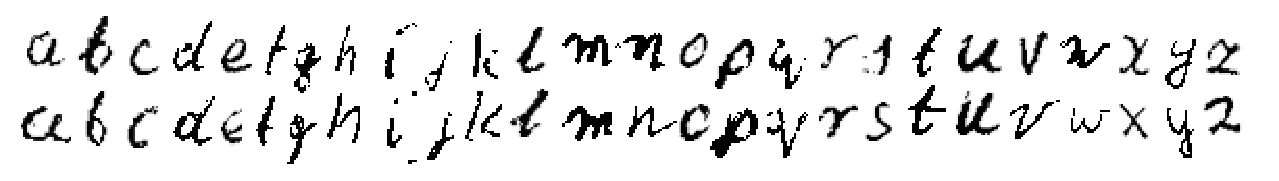
\includegraphics[width=0.7\textwidth]{_Figures/foreigns}
\vspace{-6pt}
  \caption{Sample of: native patterns (top) and foreign patterns (bottom).}
\label{fig:nativeforeignpatterns}
\vspace{-12pt}
\end{figure}

\vspace{-6pt}
%-------------------------------------------------------------------
%-------------------------------------------------------------------
\subsection{Experimental Settings}
\vspace{-3pt}

Solutions presented in this paper have been implemented in Python programming language, using scientific libraries \cite{MatLab,NumPy,Scikit}. The MVEE algorithm, available as MATLAB code  %\footnote{http://www.mathworks.com/matlabcentral/fileexchange/9542-minimum-volume-enclosing-ellipsoid/content/MinVolEllipse.m} 
has been rewritten in Python language, using NumPy library for matrix representation and operations. Several tests have been performed in order to find best suited method parameters for both classifiers and identifiers. For finding those values the Grid Search~\cite{Scikit} %\footnote{Link to Python implementation: http://scikit-learn.org/stable/modules/grid\_search.html} 
has been used for SVM and RF. % \textcolor{red}{Ellipsoids and kNN methods had their values assigned manually. }

\vspace{-9pt}
%-------------------------------------------------------------------
\subsubsection{MVEE parameters.}
Each ellipsoid was created and used with two parameters: tolerance and acceptance. The tolerance argument was used during creation phase, as ``accuracy measurement''. Lower value means that created enclosing figure is more fitted to the construction set. Acceptance parameter defines how far can a point lie outside the ellipsoid to still be identified as belonging to it. In other words, it treats enclosing ellipsoid as being bigger than it really is. Parameters tests involved computing effectiveness of MVEE algorithm for certain tolerance and acceptance values. We tested values from such ranges:\vspace{-6pt}
\begin{itemize}
	\item tolerance = [0.5, 0.2, 0.1, 0.01]
	\item accuracy = [0.1, 0.01, 0.001, 0.0005]
\end{itemize} 
The results revealed that for the given training and test sets the best parameter combination was tolerance=0.5 and accuracy=0.1 and those values were used in the final, combined method described later in this document.

\vspace{-9pt}
%-------------------------------------------------------------------
\subsubsection{SVM parameters.}
SVM method available in the Scikit package offers a few built-in kernels that were used during computations: radial basis function and polynomial. Additionally, there are two more parameters that were tested: C (described as penalty parameter C of the error term), and $\gamma$ (known as kernel coefficient). Values that were tested:\vspace{-6pt}
\begin{itemize}
	\item kernel = ['rbf', 'poly']
	\item C = [1, 2, 4, 5, 16]
	\item $\gamma = [2^{-1}, 2^{-2}, 2^{-3}, 0,00025]$
\end{itemize}
The best found combination of those parameters used rbf kernel along with C=8 and $\gamma = 2^{-1}$ values.

\vspace{-9pt}
%-------------------------------------------------------------------
\subsubsection{Random Forests parameters.}
The Scikit library was used to test random forests. Random forests with the following number of trees were tested: 1, 2, 3, 5, 10, 20, 30, 40, 50, 60, 70, 80, 90, 100, 110, 120, 130, 140, 150. It turned out that the best number of trees to build the forest was 100.

\vspace{-9pt}
%-------------------------------------------------------------------
\subsubsection{kNN parameters.}
%\textcolor{red}{The package was used for the k-NN classifier testing.}  
We tested the following values of $k$ (the number of neighbours): 1, 2, 3, 4, 5, 10, 20, 30, 40, 50. The best found value of $k$ was four. There is also one parameter -- metric, but we use the standard Euclidean metric.
%TODO jaki pakiet?

\vspace{-9pt}
%-------------------------------------------------------------------
%-------------------------------------------------------------------
%\subsection{Concept of Classification with Rejection}
\subsection{Results of Experiments}
\vspace{-3pt}

In this section we present the results of our experiments. We use quality measures presented in Section~\ref{subsec:QualityEvaluation}. We investigate classification quality, rejection quality and rejection's impact on classification quality. We compare two scenarios: global (rejection on is the entire dataset) and local (rejection mechanism is separate for each native class). 

\vspace{-12pt}
%-------------------------------------------------------------------
\subsubsection{Influence of Rejection on Native Patterns Classification}
Adding a~rejection mechanism, ideally, may be a~method for improvement of classification rates. It would be perceived as a~positive side of the rejection mechanism, if it would be able to reject those native patterns, which would be incorrectly classified when there is no rejection mechanism at all. 

\begin{table}[!b]
\vspace{-12pt}
\centering
\caption{Classification with random forests, svms and knn and rejection with ellipsoids on the set of native patterns: no rejection vs. local and global rejections. Notice that all three measures turn to the same proportion CC/TP for no rejection mode.}
\vspace{-6pt}
\setlength{\tabcolsep}{3pt}
\renewcommand{\arraystretch}{1}
{\footnotesize
\begin{tabular}{|r||c|c|c||c|c|c||c|c|c|}
\hline
& \multicolumn{3}{c||}{No rejection} & \multicolumn{3}{c||}{Global rejection} & \multicolumn{3}{c|}{Local rejection}\\
\hline
  Basic Classifier & $\;\;$RF$\;\;$ & $\,$SVM$\,$ & kNN & $\;\;$RF$\;\;$ & $\,$SVM$\,$ & kNN & $\;\;$RF$\;\;$ & $\,$SVM$\,$ & kNN  \\
  \hline
  Data Set & \multicolumn{9}{c|}{Native Patterns, Train Set} \\
\hline
Strict Accuracy     & $1$ & $0.985$ & $0.955$ & $0.941$ & $0.938$ & $0.936$ & $0.942$ & $0.942$ & $0.942$ \\
Fine Accuracy       & $1$ & $0.985$ & $0.955$ & $1$     & $0.987$ & $0.972$ & $1$ & $0.989$ & $0.984$ \\
Strict Native Sens. & $1$ & $0.985$ & $0.955$ & $0.879$ & $0.852$ & $0.854$ & $0.864$ & $0.857$ & $0.845$ \\
\hline
Data Set & \multicolumn{9}{c|}{Native Patterns, Test Set} \\
\hline
Strict Accuracy  & $0.952$ & $0.966$ & $0.930$ & $0.946$ & $0.946$ & $0.944$ & $0.951$ & $0.952$ & $0.953$ \\
Fine Accuracy       & $0.952$ & $0.966$ & $0.930$ & $0.972$ & $0.982$ & $0.959$ & $0.977$ & $0.985$ & $0.976$ \\
Strict Native Sens. & $0.952$ & $0.966$ & $0.930$ & $0.842$ & $0.852$ & $0.831$ & $0.837$ & $0.845$ & $0.825$ \\
\hline
\end{tabular}
}
\vspace{-6pt}
\label{tab:NativeNoForeign}
\end{table}

Trained models partially fulfill this wish. Conducted tests, reported in Table \ref{tab:NativeNoForeign}, show that Fine Accuracy improved for both local and global rejection schemes and for all classifiers. This means that we have a better recognition rate (the proportion of correctly classified patterns) in the data that was accounted as native. However, we have to notice that both rejection mechanisms rejected some native patterns. Hence, Strict Accuracy and Strict Native Sensitivity are slightly higher when we do not have any rejection mechanism.

Results indicate that performing pattern rejection after their initial classification (the local rejection scheme), brings better results than using the global scheme. This could be explained by the fact that in the local rejection scheme we use one ellipsoid per each class and we apply those ellipsoids after classification. In contrast, in the global scheme we have a~joint set of ellipsoids that we apply to the entire dataset. In the local rejection scenario native patterns identification regions are applied individually to each subset obtained from the classifier. As a~result there is a chance that classification would contribute to foreign patterns filtration. The same conclusion, about superiority of local rejection over global one concerns strict classification error ratios.

When comparing the overall quality achieved by mechanisms based on different classifiers we see a slight advantage of SVM. 

\vspace{-12pt}
%-------------------------------------------------------------------
%-------------------------------------------------------------------
\subsubsection{Separating Letters from Digits}
Figure \ref{fig:Measures} presents rejection results. We compare various quality measures for models constructed based on random forests, SVM, and kNN with ellipsoids for the global and the local rejection schemes. 

\begin{figure}[!t]
\vspace{-12pt}
  \centering
  \includegraphics[width=\textwidth]{_Figures/Measures_BW.png}\\
  \caption{Quality evaluation for global and local rejection schemes realized with ellipsoids with different classifiers: random forests, SVMs, and kNNs.}
\label{fig:Measures}
\vspace{-12pt}
\end{figure}

First, let us mention that for the global rejection all rejection rates are the same for all classifiers. This is due to the specificity of this model, where rejection occurs first, so classification procedure does not modify the content of the set subjected to rejection. However, the global approach turned out to be slightly worse than the local approach. 

Results show that in the local rejection model all classifiers combined with ellipsoids behave well and provide similar quality of rejection.   

\vspace{-6pt}
%-------------------------------------------------------------------
%-------------------------------------------------------------------
%-------------------------------------------------------------------
\section{Conclusions}
  \label{sec:Conclusion}
\vspace{-3pt}

Enhancing classifiers' ability to classify objects by coupling them with ellipsoids for foreign patterns rejection has proven to yield good results. Conducted experiment on handwritten digits contaminated with handwritten letters showed that  the local rejection scenario with fine-grained rejection ellipsoids one per each native class perform better than the global approach with a single, but less fine-grained rejection mechanism. We also report that the differences in classification ratios in the local rejection model coupled with different classifiers turned out to be very slight. SVM turned out to be the best, and its advantage is visible when we evaluate the rate of native patterns that were rejected that wanted to reject, because otherwise they would have been classified into incorrect class.

We are aware that to truly confirm obtained results, test should be repeated on different data sets. Described in this paper set consisting of letters and digits, although being very large, might not match wide spectrum of problems.  %consist of enough distinguishable classes.

Let us conclude this paper by saying that various adaptations of the idea of foreign patterns rejection have a vital role in modern machine learning. It is needless to mention areas such as text mining, fraud detection, or medical diagnosis systems where we deal with various reincarnations of the foreign patterns. From this perspective we believe that the study in this direction is worth further efforts.

\vspace{-6pt}
%-------------------------------------------------------------------
%-------------------------------------------------------------------
%-------------------------------------------------------------------
\section*{Acknowledgment}
\vspace{-5pt}
The research is partially supported  by the National Science Center, grant No 2012/07/B/ST6/01501, decision no \mbox{DEC-2012/07/B/ST6/01501}.


\vspace{-6pt}
%-------------------------------------------------------------------
%-------------------------------------------------------------------
%-------------------------------------------------------------------
\begin{thebibliography}{19}
\vspace{-3pt}

\bibitem{Altman1992}
Altman N. S., \emph{An introduction to kernel and nearest-neighbor nonparametric regression}. The American Statistician 46 (3), 1992, pp. 175-185.

\bibitem{BertolamiZimmermannBunke2006}
Bertolami, R., Zimmermann, M., Bunke, H., \emph{Rejection strategies for offline handwritten text line recognition}, Pattern Recogn. Letters 27(16), 2006, pp. 2005-2012.

\bibitem{Breiman2001}
Breiman, L., \emph{Random Forests}. Machine Learning 45 (1), 2001, pp. 5-32. 

\bibitem{BurgerKessentiniPaquet2011}
Burger, T., Kessentini, Y., Paquet, T., \emph{Dempster-Shafer based rejection strategy for handwritten word recognition}, Proc. of the 2011 International Conference on Document Analysis and Recognition, 2011, pp. 528-532.

\bibitem{CortesVapnik1995}
Cortes, C., Vapnik, V., \emph{Support-vector networks}. Machine Learning 20 (3), 1995, pp. 273-297.
 
\bibitem{EladHel-OrKeshet2001}
Elad, M., Hel-Or, Y., Keshet, R., \emph{Pattern detection using maximal rejection classiffier}, C. Arcelli et al. (Eds.): Proc. International Workshop on Visual Form, Lecture Notes on Computer Science 2059, 2001, pp. 514-524.
 
\bibitem{HempstalkFrankWitten2008}
Hempstalk, K. et al., \emph{One-class classification by combining density and class probability estimation}, Machine Learn. and Knowl. Disc. in Databases, 2008, pp. 505-519.

\bibitem{HomendaICAART2015}
Homenda, W., Jastrzebska, A., Pedrycz, W., \emph{Rejecting Foreign Elements in Pattern Recognition Problem. Reinforced Training of Rejection Level}, in: Proc. of ICAART 2015, 2015, pp. 90-99.

%\bibitem{IglewiczHoaglin1993}
%Iglewicz B., Hoaglin D., \emph{How to Detect and Handle Outliers},  Milwaukee: ASOC Quality Press, 1993.

\bibitem{LeCunCortesBurges}
LeCun, Y., Cortes, C., and Burges, C., \emph{The MNIST database of handwritten digits}, in: http://yann.lecun.com/exdb/mnist.

\bibitem{Romanski}
Romanski, P., Kotthoff, L., \emph{Package FSelector}, http://cran.r-project.org/web/packages/FSelector/FSelector.pdf

\bibitem{SchemeHudginsEnglehart2013}
Scheme, E. J., Hudgins, B. S., Englehart, K. B., \emph{Confidence-based rejection for improved pattern recognition myoelectric control}, IEEE Trans. Biomed. Eng. 60(6), 2013, pp. 1563-1570.

\bibitem{ScholkopfWilliamsonSmola1992}
Scholkopf, B., Williamson, R., Smola, A., Shawe-Taylort, J., Platt, J., \emph{Support Vector Method for Novelty Detection}, Advances in Neural Information Processing Systems 12, 1992, pp. 582-588. 

\bibitem{TaxDuin2008}
Tax, D. M. J., Duin, R. P. W., \emph{Growing a multi-class classifier with a reject option}, Pattern Recognition Letters 29, 2008, pp. 1565-1570.

\bibitem{MVEEMichaelTodd2005}
Todd, M. J., Yildirim, E. A., \emph{On Khachiyan's Algorithm for the Computation of Minimum Volume Enclosing Ellipsoids}, September 30, 2005, article link: http://people.orie.cornell.edu/miketodd/TYKhach.pdf

\bibitem{WangCasasent2009}
Wang, Y., Casasent, D., \emph{A Support Vector Hierarchical Method for multi-class classification and rejection}, Proc. of Int. Joint Conf. on Neural Networks, 2009, pp. 3281-3288.

\bibitem{MatLab}
http://www.mathworks.com/

\bibitem{NumPy}
http://www.numpy.org/

\bibitem{Scikit}
http://scikit-learn.org/stable/

%\bibitem{ScikitSVM}
%http://scikit-learn.org/stable/modules/generated/sklearn.svm.SVC.html [2016, 3 April]
	
%\bibitem{ScikitRF}
%http://scikit-learn.org/stable/modules/generated/sklearn.ensemble.RandomForestClassifier.html [2016, 3 April]

%\bibitem{ScikitKNN}
%http://scikit-learn.org/stable/modules/generated/sklearn.neighbors.KNeighborsClassifier.html [2016, 3 April]
 
\end{thebibliography}

\end{document}


%-------------------------------------------------------------------
%-------------------------------------------------------------------
%\subsection{Concept of Classification with Rejection}
\subsection{Results of Experiments}
  \label{subsec:ClassificationAndRejection}

To determine effectiveness of parameter values for each method, confusion matrix has been calculated. Each row of this matrix represents information about distribution of patterns from certain class. For instance, 213 zeros were correctly classified to their class, four zeros were incorrectly classified as ones, two zeros -- as sixes, 17 zeros as eights and 58 zeros were incorrectly rejected as non-digit patters, cf. row ``0'' in Table~\ref{tab:CofusionTable}. Numbers in each column hold information about quantity of patterns that were classified as belonging to the corresponding class.

\begin{table*}[h]
\centering
\caption{Confusion table for SVM with global rejection on training set }
\vspace{-3pt}
\setlength{\tabcolsep}{3pt}
\renewcommand{\arraystretch}{1}
{\footnotesize
\begin{tabular}{|c||r|r|r|r|r|r|r|r|r|r|r|}
\hline
 \hspace{15pt} & $0\;\;\;$ & $1\;\;\;$ & $2\;\;\;$ & $3\;\;\;$ & $4\;\;\;$ & $5\;\;\;$ & $6\;\;\;$ & $7\;\;\;$ & $8\;\;\;$ & $9\;\;\;$ & $f$ \\
\hline\hline
  0 & 595 &  &   &   &   &   & 1 &   & 10 &   & 80\\
\hline
  1 &  & 670 & 1 &   &   &   & 1 &   &   &   & 122\\
\hline
  2 &  &   & 641 &   &   &   &   & 1  &   & 1  & 79\\
\hline
  3 &  &   & 3 & 629 &   & 1 &   & 2 &  &   & 72\\
\hline
  4 &  &   &   &   & 598 &   &   &  &  & 7 & 82\\
\hline
  5 &  &   &   & 6 &  & 546 &   &   & 4 &   & 68\\
\hline
  6 & 1 & &   &   &   &   & 567 &   & 1 &   & 102\\
\hline
  7 &  & 1  &  & 1 & 1 &   &   & 626 &   & 5 & 85\\
\hline
  8 & 8 &   &   &   & 2 &   &   & 1 & 589 & 2 & 79\\
\hline
  9 &  & 1 &  & 4 & 3 & 2 &   & 6 & 4 & 607 & 79\\
\hline
$f$ & 181 & 44 & 155 & 16 & 164  & 104 & 182 & 9 & 211 & 61 & 25256\\
\hline
\end{tabular}
}
\vspace{-3pt}
\label{tab:CofusionTable}
\end{table*}


\begin{table}[!ht]
\centering
\caption{Results of classification with rejection on the set of native patterns supplemented with different sets of semi-synthetic foreign patterns
%.... \color{red}Moze na razie wstrzymajmy si� z semi-synthetic, poniewaz wymgaloby to rozszerzenia zakresu obliczen. Sprobujmy uporzadkowac i ewentualnie uzupelnic otrzymane dane bazujac na dotyczasowych danych: cyfrach i literach, tak uzupelnic, by uzyskac mozliwie najwiecej wnioskow.
}
%\vspace{3pt}
\setlength{\tabcolsep}{4pt}
\renewcommand{\arraystretch}{1}
\begin{tabular}{|r||c|c|c||c|c|c|}
\hline
  Data Set & \multicolumn{3}{c||}{ Global rejection } & \multicolumn{3}{c|}{ Local Rejection } \\
\hline
  Basic Classifier & RF & SVM & KNN &  RF & SVM & KNN  \\
\hline
Accuracy            & 0.944 & 0.944 & 0.944 & 0.947 & 0.948 & 0.950 \\
Strict Accuracy     & 0.943 & 0.942 & 0.940 & 0.946 & 0.947 & 0.947 \\
Fine Accuracy       & 0.992 & 0.986 & 0.968 & 0.993 & 0.988 & 0.981 \\
Native Precision    & 0.795 & 0.795 & 0.795 & 0.818 & 0.821 & 0.835 \\
Native Sensitivity  & 0.875 & 0.875 & 0.875 & 0.862 & 0.864 & 0.855 \\
Strict Native Sens. & 0.868 & 0.863 & 0.847 & 0.856 & 0.854 & 0.839 \\
Foreign Precision   & 0.976 & 0.976 & 0.976 & 0.974 & 0.974 & 0.972 \\
Foreign Sensitivity & 0.957 & 0.957 & 0.957 & 0.964 & 0.964 & 0.968 \\
Native F-measure    & 0.833 & 0.833 & 0.833 & 0.839 & 0.842 & 0.845 \\
Foreign F-measure   & 0.966 & 0.966 & 0.966 & 0.969 & 0.969 & 0.970 \\
\hline
\end{tabular}
%\vspace{12pt}
\label{tab:rejection_results}
\end{table}
%{\color{blue}
